% Généré par analysis/analyse.py -- ne pas modifier à la main.
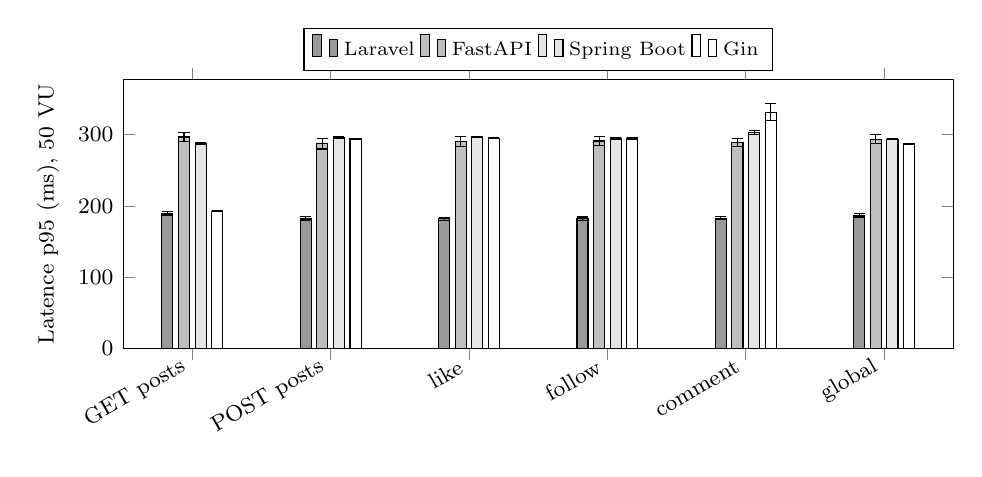
\begin{tikzpicture}
\begin{axis}[
  width=\columnwidth, height=5cm,
  ybar, bar width=4pt, ymin=0,
  symbolic x coords={GET posts,POST posts,like,follow,comment,global},
  xtick=data,
  x tick label style={rotate=30, anchor=east},
  ylabel={Latence p95 (ms), 50~VU},
  tick label style={font=\footnotesize},
  label style={font=\footnotesize},
  legend style={font=\scriptsize, at={(0.5,1.03)}, anchor=south, legend columns=4},
  enlarge x limits=0.1,
  enlarge y limits={upper, value=0.1}]
\addplot[fill=gray!80, draw=black, error bars/.cd, y dir=both, y explicit]
  coordinates {(GET posts,189.67) +- (0,2.37) (POST posts,182.42) +- (0,2.20) (like,181.93) +- (0,2.14) (follow,182.13) +- (0,2.38) (comment,182.89) +- (0,2.28) (global,186.77) +- (0,2.26)};
\addplot[fill=gray!50, draw=black, error bars/.cd, y dir=both, y explicit]
  coordinates {(GET posts,296.60) +- (0,6.85) (POST posts,287.47) +- (0,7.66) (like,290.67) +- (0,7.04) (follow,291.02) +- (0,6.28) (comment,289.52) +- (0,5.64) (global,293.79) +- (0,6.64)};
\addplot[fill=gray!20, draw=black, error bars/.cd, y dir=both, y explicit]
  coordinates {(GET posts,287.69) +- (0,1.63) (POST posts,295.62) +- (0,1.43) (like,296.81) +- (0,0.92) (follow,294.51) +- (0,1.65) (comment,303.25) +- (0,2.86) (global,293.65) +- (0,0.95)};
\addplot[fill=white, draw=black, error bars/.cd, y dir=both, y explicit]
  coordinates {(GET posts,192.45) +- (0,0.58) (POST posts,294.16) +- (0,0.88) (like,295.18) +- (0,0.90) (follow,294.93) +- (0,1.09) (comment,331.64) +- (0,11.46) (global,286.87) +- (0,1.08)};
\legend{Laravel, FastAPI, Spring Boot, Gin}
\end{axis}
\end{tikzpicture}
